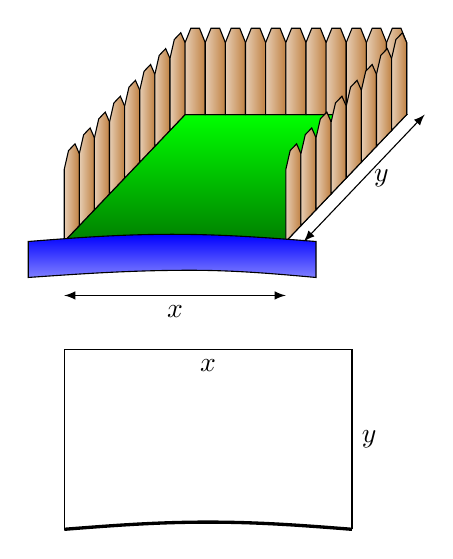
\begin{tikzpicture}[scale=1.3]

\shadedraw [top color = green,bottom color = green!50!black] (0,0) -- (33.6pt,35.28pt) -- (95.2pt,35.28pt) -- (61.6pt,0) -- cycle;

\begin{scope}[cm={1,1.05,0,1,(0,0)}]
\foreach \x in {0,...,7}
	{
	\shadedraw [xscale=.3,shift={(\x*14 pt,0)},left color=brown!40!white,right color = brown!99!white] (0,0) -- 	++(0,20pt)  -- ++(4pt,4pt)  -- ++(6pt,0pt) -- ++(4pt,-4pt)-- ++(0pt,-20pt) -- cycle;
	}
\end{scope}

\begin{scope}[shift={(33.6pt,35.28pt)}]
\foreach \x in {0,...,10}
	{
		\shadedraw [xscale=.4,shift={(\x*14 pt,0)},left color=brown!40!white,right color = brown!99!white] (0,0) -- 	++(0,20pt)  -- ++(4pt,4pt)  -- ++(6pt,0pt) -- ++(4pt,-4pt)-- ++(0pt,-20pt) -- cycle;
	}
\end{scope}
	
\begin{scope}[cm={1,1.05,0,1,(61.6pt,0)}]
\foreach \x in {0,...,7}
	{
	\shadedraw [xscale=.3,shift={(\x*14 pt,0)},left color=brown!40!white,right color = brown!99!white] (0,0) -- 	++(0,20pt)  -- ++(4pt,4pt)  -- ++(6pt,0pt) -- ++(4pt,-4pt)-- ++(0pt,-20pt) -- cycle;
	}
\end{scope}

\shadedraw [top color=blue, bottom color=blue!50!white] (-10pt,0) sin (30pt,2pt) cos (70pt,0pt) -- (70pt,-10pt) sin (35pt,-8pt) cos (-10pt,-10pt) --cycle;

%\foreach \x in {0,...,10}
%	{
%		\shadedraw [xscale=.4,shift={(\x*14 pt,0)},left color=brown!40!white,right color = brown!99!white] (0,0) -- 	++(0,20pt)  -- ++(4pt,4pt)  -- ++(6pt,0pt) -- ++(4pt,-4pt)-- ++(0pt,-20pt) -- cycle;
%	}

\draw [<->,>=latex] (0,-15pt) -- (61.6pt,-15pt) node [below,pos=.5] {$x$};
\draw [<->,>=latex] (100.2pt,35.28pt) -- (66.6pt,0pt) node [right,pos=.5] {$y$};

\draw [shift = {(0,-80pt)}] (0,0) -- (0,50pt) -- (80pt,50pt) node [pos=.5,below] {$x$} --(80pt,0) node [pos=.5,right] {$y$};
\draw [{\colorone},very thick,shift = {(0,-80pt)}] (0,0) sin (40pt,2pt) cos (80pt,0);

\end{tikzpicture}